\documentclass{beamer}
\usepackage{listings}
\usepackage{amsmath,amssymb,amsfonts}
\usepackage{graphicx}
\usepackage{hyperref}
\usepackage{textcomp}
\usepackage{xcolor}
\usepackage{algorithm}
\usepackage{algorithmic}
\usepackage{geometry}
\usepackage{array}


\title{Group 3: LDPC codes in Memory}
\author{Tom Wang \\ Natalie Balashov}
\date{April 10th, 2024}

\begin{document}

\begin{frame}
    \titlepage
\end{frame}

% \begin{frame}{Intro}
%     Example of lists with Roman numerals:
%     \begin{enumerate}[I]
%         \item Point A
%         \item Point B
%               \begin{enumerate}[i]
%                   \item part 1
%                   \item part 2
%               \end{enumerate}
%         \item Point C
%         \item Point D
%     \end{enumerate}
% \end{frame}
% 
% \begin{frame}{Using Columns}
%     \begin{columns}
%         \column{0.5\textwidth}
%         column 1 with background info
%         \column{0.5\textwidth}
%         column 2 with more background info
%     \end{columns}
% \end{frame}
% 
% \begin{frame}{Pictures with text below}
%     % \begin{figure}
%     %     \includegraphics[scale=0.1]{figures/image_name.png}
%     %     \caption{A sample figure}
%     % \end{figure}
%     Insert explanatory text here.
% \end{frame}
% 
% \begin{frame}{Pictures with text beside}
%     \begin{columns}
%         \column{0.5\textwidth}
%         column 1 with background info
%         \column{0.5\textwidth}
%         % \begin{figure}
%         %     \includegraphics[scale=0.1]{figures/figure_name.png}
%         %     \caption{A sample figure}
%         % \end{figure}
%     \end{columns}
% \end{frame}
% 
% \begin{frame}{Lists in Beamer}
%     This is an unordered list:
%     \begin{itemize}
%         \item Item 1
%         \item Item 2
%         \item Item 3
%     \end{itemize}
%     and this is an ordered list:
%     \begin{enumerate}
%         \item Item 1
%         \item Item 2
%         \item Item 3
%     \end{enumerate}
% \end{frame}
% 
% \begin{frame}{Blocks in Beamer}
%     \begin{block}{Standard Block}
%         This is a standard block.
%     \end{block}
%     \begin{alertblock}{Alert Message}
%         This block presents alert message.
%     \end{alertblock}
%     \begin{exampleblock}{An example of typesetting tool}
%         Example: MS Word, \LaTeX{}
%     \end{exampleblock}
% \end{frame}
% 
% \begin{frame}{Math Blocks in Beamer}
%     \begin{definition}
%         A prime number is a number that...
%     \end{definition}
%     \begin{theorem}[Pythagoras]
%         $a^2 + b^2 = c^2$
%     \end{theorem}
%     \begin{corollary}
%         $x + y = y + x  $
%     \end{corollary}
%     \begin{proof}
%         $\omega +\phi = \epsilon$
%     \end{proof}
% \end{frame}
% 
% \begin{frame}[fragile]{Including Code}
%     \begin{semiverbatim}
%         \\begin\{frame\}
%         \\frametitle\{Outline\}
%         \\tableofcontents
%         \\end\{frame\}
%     \end{semiverbatim}
%     \begin{semiverbatim}
%         int function() \{
%         int i = 0;
%         return i * i;
%         \}
%     \end{semiverbatim}
% \end{frame}
% 
% \begin{frame}{Table example}
%     \begin{table}
%         \begin{tabular}{l | c | c | c | c }
%             Competitor Name & Swim  & Cycle & Run   & Total \\
%             \hline \hline
%             John T          & 13:04 & 24:15 & 18:34 & 55:53 \\
%             Norman P        & 8:00  & 22:45 & 23:02 & 53:47 \\
%             Alex K          & 14:00 & 28:00 & n/a   & n/a   \\
%             Sarah H         & 9:22  & 21:10 & 24:03 & 54:35
%         \end{tabular}
%         \caption{Triathlon results}
%     \end{table}
% \end{frame}

\begin{frame}{Overview}
    \begin{enumerate}
        \item Intro to LDPC Codes
        \item Implementation of LDPC Codes in HDL
        \item Implementation of Hamming Codes in HDL
        \item Comparison of LDPC and Hamming Codes
    \end{enumerate}
\end{frame}

\begin{frame}{Hamming implementation}
  \begin{itemize}
    \item Typical Hamming codes in implementation uses 64-bit to 72-bit encoding schemes.
    \item This typical implementation is called \textbf{SECDED} (Single Error Correction,
    Double Error Detection) Hamming code.
    \item The concept of Hamming code is detecting errors in half of the codewords.
      And then with different combinations of deleting patterns, we can locate a single
    bit.
  \end{itemize}
  \begin{figure}[htbp]
    \centerline{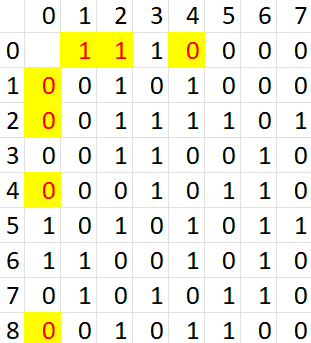
\includegraphics[scale = 0.6]{Images/Hamming_example.png}}
    \caption{Parity bits and data bits in a Hamming code.}
  \end{figure}
\end{frame}

\begin{frame}{Example of correcting error}
    There are a total of 72 bits, which can be expressed in binary from $6'b000\_0000$ to $6'b 100\_0111$.

    Mark the unique position vector as \texttt{vec[6:0]} and let it be bijective to
    parity bits \texttt{p[6:0]}.

    We order the bits as shown below:

    \begin{figure}[htbp]
        \centerline{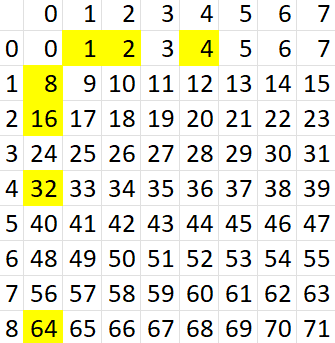
\includegraphics[scale = 0.6]{Images/Hamming_bits_order.png}}
        \caption{Number parity bits and data bits in a Hamming code.}
    \end{figure}
\end{frame}

\begin{frame}{FPGA Implementation}
    Logic can be easily achieved with a series of \textit{xor gates} and \textit{and gates}.

    RTL viewer can be found on GitHub for \href{https://github.com/luckunately/ELEC433-Projects/blob/add-tex/Hamming72out/Hamming72out_RTL.pdf}{Hamming72out} and \href{https://github.com/luckunately/ELEC433-Projects/blob/add-tex/Hamming64in/Hamming64inRTL.pdf}{Hamming64in}.

    According to Quartus timing analysis, the highest frequency it can run is
    \textbf{387.3 MHz} under \textit{slow 1100 mV 85C mode}.

    \begin{itemize}
      \item Combinational ALUT usage for logic: 154
      \begin{itemize}
        \item 7 input functions: 0
        \item 6 input functions: 121
        \item 5 input functions: 10
        \item 4 input functions: 13
        \item $\leq$ 3 input functions: 10
      \end{itemize}
      \item Dedicated logic registers: 69
    \end{itemize}
\end{frame}

\begin{frame}{LDPC pareity check matrix}
    To achieve the similar behavior of Hamming code, we will use a $64-72$ LDPC code which has parameters $n=72, j=4, i=36$.

    There are lots of possible parity check matrices, the one we will use would be linked in our GitHub \href{https://hichamjanati.github.io/pyldpc/}{GitHub repo} since it is too large to be included in this report. This is generated by a Python library called \href{https://hichamjanati.github.io/pyldpc/}{\texttt{pyldpc}}

    \begin{figure}[htbp]
      \centerline{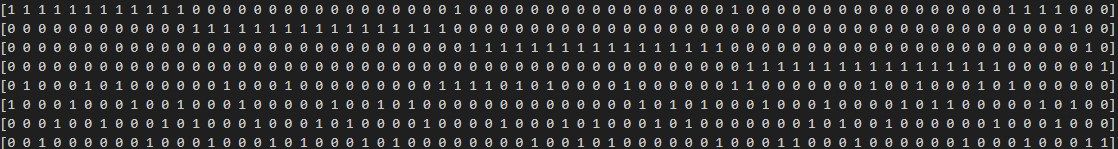
\includegraphics[scale = 0.4]{Images/LDPC_Parity_Matrix.jpg}}
      \caption{8x72 Parity check matrix for LDPC code.}
  \end{figure}
    
\end{frame}

\begin{frame}{Generator matrix}
    Similar to Hamming code, the message bits are directly passed to the encoder with additional 8 parity bits.

    To generate the generator matrix, we can use the following algorithm:
    \begin{enumerate}
      \item Assume that the encoded code $c$ of length $n$ is composed of the parity bits
            $b$ and the message bits $m$ in a form $c = [b, m]$.
      \item Then if there are no errors in the code, $cH^T = [b, m]H^T = 0$.
      \item Divide $H$ into $H = [H_1, H2]^T$ where $H_1$ is a square matrix of size $n-k$.
            Note that $b$ is of length $n-k$ as well. So we can break the matrix
            multiplication into $[b, m][H_1, H_2]^T = bH_1^T + mH_2^T = 0$.
      \item Since we are in a binary field, $bH_1^T = mH_2^T \implies b =
              mH_2^T(H_1^T)^{-1}$. Name the matrix $H_2^T(H_1^T)^{-1}$ as $A$.
      \item So the generator matrix $G$ is $[A, I_{n-k}]$.
    \end{enumerate}
\end{frame}

\begin{frame}{Decoding algorithm}
  A recursive algorithm called \textbf{bit-flipping} is used to decode the LDPC code.

  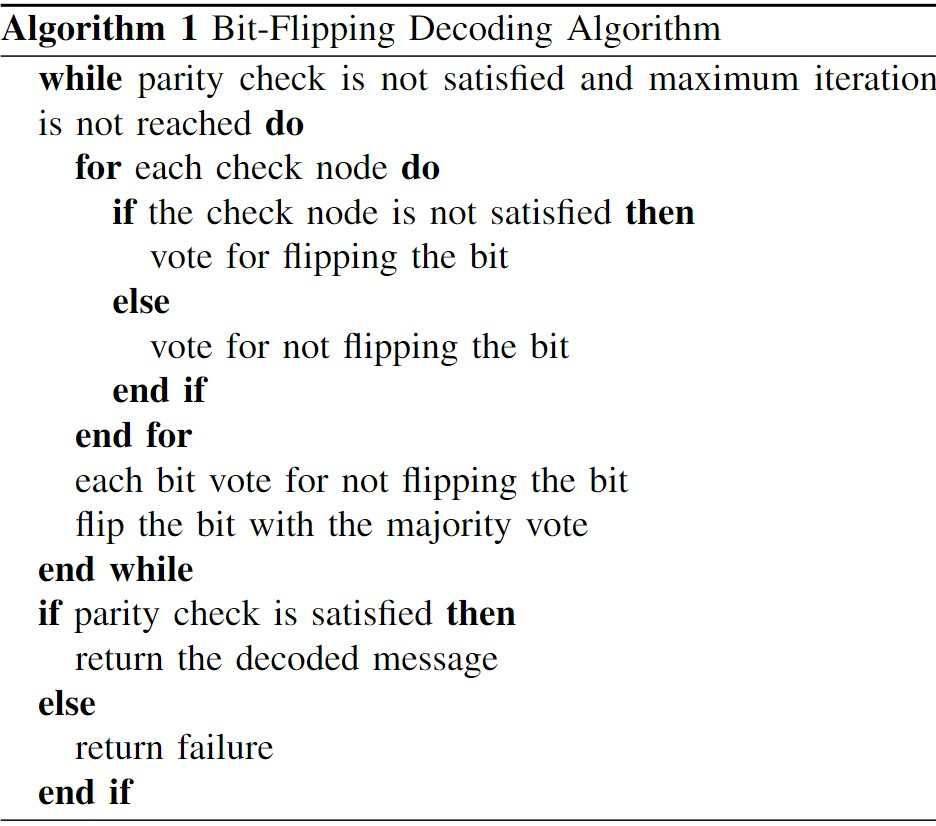
\includegraphics[scale=0.3]{Images/Bit_Flipping_Algorithm.jpg}

  % For some reason it does not compile, use image for now
  % \begin{algorithm}
  %   \caption{Bit-Flipping Decoding Algorithm}
  %   \begin{algorithmic}
  %     \WHILE{parity check is not satisfied and maximum iteration is not reached}
  %       \FOR{each check node}
  %         \IF{the check node is not satisfied}
  %           \STATE vote for flipping the bit
  %         \ELSE
  %           \STATE{vote for not flipping the bit}
  %         \ENDIF
  %       \ENDFOR
  %       \STATE each bit vote for not flipping the bit
  %       \STATE flip the bit with the majority vote
  %     \ENDWHILE
  %     \IF {parity check is satisfied}
  %     \STATE return the decoded message
  %     \ELSE
  %     \STATE return failure
  %     \ENDIF
  %   \end{algorithmic}
  % \end{algorithm}
\end{frame}

\begin{frame}{Performance}
  % Will explain what this is verbally, too much info is not good on slides
  On DE1-SOC, Quartus analysis shows that the highest frequency it can run is \textbf{325.73 MHz} under \textit{slow 1100 mV 85C mode}.

  \begin{itemize}
    \item Combinational ALUT usage for logic: 114 \begin{itemize}
      \item 7 input functions: 0
      \item 6 input functions: 4
      \item 5 input functions: 10
      \item 4 input functions: 28
      \item $\leq$ 3 input functions: 72
    \end{itemize}
    \item Dedicated logic registers: 72
  \end{itemize}
\end{frame}

\begin{frame}{Comparison}
  Although the Hamming code has a higher frequency, the LDPC code has a lower ALUT usage and more dedicated logic registers. This means that the LDPC code is more efficient in terms of hardware usage.

Also, the frequency difference is not that significant. On ASIC designs, the story might be different. 
  \begin{table}[htbp]
    \centering
    \caption{Comparison of Decoding Algorithms}
    \label{tab:decoding_comparison}
    \begin{tabular}{|l|c|c|}
      \hline
      \textbf{Parameter} & \textbf{Hamming} & \textbf{LDPC} \\
      \hline
      Highest Frequency (MHz) & 387.3 & 325.73 \\
      \hline
      ALUT Usage for Logic & 154 & 114 \\
      \quad 7 input functions & 0 & 0 \\
      \quad 6 input functions & 121 & 4 \\
      \quad 5 input functions & 10 & 10 \\
      \quad 4 input functions & 13 & 28 \\
      \quad $\leq$ 3 input functions & 10 & 72 \\
      \hline
      Dedicated Logic Registers & 69 & 72 \\
      \hline
    \end{tabular}
  \end{table}
\end{frame}


\end{document}
